\chapter{Conclusions and Future Work}\label{ch:conclusion}
\section{Summary}

\section{Thesis Contribution}

\section{Recommendations for Future Work}\label{ch:future}
***************************************\\
Model Validation\\

***************************************\\
\subsection{Modeling Constraints}
There are several techniques to handle input saturation, the most popular ones are anti-windup techniques. Back-calculation is such a method for PID to activate the integrator, is this possible for NL control?

\subsection{Hybrid Modeling}
Switching between several flight modes yields autonomous acrobatic maneuvers. Robust to switching conditions ***why?\\
\begin{figure}[h!]
	\centering
	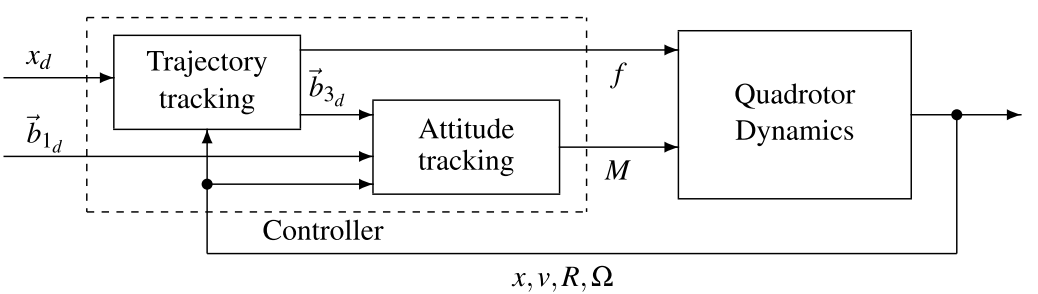
\includegraphics[width=.45\textwidth]{./StyleStuff/LeeControlscheme.png}
	\caption{\label{fig:}}
\end{figure}		

\subsection{Trajectory Generation}
\subsubsection{Minimum Snap Trajectory Generation}

Trajectory can be generated by solving a \a{QP} via minimum snap generation.

Problem in smaller space with help of differential flatness.

Is able to include constraints.
